\documentclass[a4paper, 10pt]{book}

\usepackage{tcolorbox}

\usepackage{wrapfig}

\usepackage{graphicx}
\usepackage{float}

\usepackage{tikz}
\usepackage{amsmath}

\usepackage{fontspec} % --fontspec-- package to use other fonts
\setmainfont{Vazirmatn-Regular.ttf} 
\newfontfamily\bold{Vazirmatn-Bold.ttf}

\usepackage{hyperref}

\usepackage{color}

\usepackage{geometry}
\geometry{top=2cm, bottom=2cm, left=1.5cm, right=1.5cm}

\title{\huge {\bold Parallel Algorithms}}
\author{Professor\\{\bold Dr. Masoumeh Damroudi}}
\date{Author\\{\bold Mohammad Khorshidi}}

\linespread{1.3}

\begin{document}

    \pagenumbering{roman}
    \maketitle
    \newpage

    \begin{center}
        \Large {\bold Course Overview}
    \end{center}

    In this lecture note, I have documented my personal interpretations and understanding of the material. Please note that there may be inaccuracies, and it is recommended to consult primary and authoritative sources for complete and accurate information. Additionally, I welcome any contributions to improve and refine this note. If you are reading this and would like to offer suggestions, feel free to do so via pull requests on my \href{https://github.com/elprofesorsunny/Master/tree/main/Papers/Parallel%20Aalgorithms/Booklet}{\textcolor{blue}{\bold GitHub}} or by emailing me at \href{mailto:someone@somewhere.com}{\textcolor{blue}{\bold mohammad\_khorshidi@outlook.fr}}.

    \section{Course Structure}

    \section{Instructor's Approach}

    \section{Grading and Evaluation}

        The grading structure for this course is as follows, with students expected to earn their grades based on the criteria outlined below:

        \begin{itemize}
            
            \item {\bold Presentation:} 4 points will be awarded for presenting and explaining a paper related to one aspect of parallelization, accompanied by its relevant implementation.

            \item {\bold Midterm Exam:} 4 points will be given for the midterm exam.

            \item {\bold Final Exam:} 12 points will be awarded for the final exam.

        \end{itemize}

        Additionally, students are expected to attend all classes and give due attention to the assignments that will be provided throughout the semester.
        
    \section{Course Materials and Resources}

    \tableofcontents
    
    \chapter{{\bold Introduction}}

    \pagenumbering{arabic}

        In today’s world, with the increasing volume of data and the need for faster computations, parallel algorithms have emerged as an effective method to enhance the performance of computing systems. Parallel algorithms allow us to divide a problem into smaller sub-problems, each of which can be processed simultaneously by multiple processors. This not only speeds up processing but also optimizes the use of hardware resources.

        In this lecture note, we will explore fundamental concepts of parallel processing, computational models such as the PRAM model, and interconnection structures like network links. We will also delve into the principles of designing and analyzing parallel algorithms, covering key metrics such as performance, speedup, and scalability. Our goal is to provide a comprehensive understanding of the challenges and opportunities in the field of parallel algorithms.

        Parallel algorithms play a crucial role in improving the performance of complex and resource-intensive computations. The primary goal of parallel algorithms is to divide a large problem into smaller, independent sub-problems, which can be solved simultaneously by multiple processors. This technique is essential in multi-core and distributed computing environments such as supercomputers and large computing clusters.

        The need for parallel computation arises from the requirement to process large amounts of data or perform complex computations in a reasonable amount of time. A parallel computer, which consists of multiple processing units or processors, enables this by dividing a large problem into smaller sub-problems. Each of these sub-problems is solved independently and simultaneously by separate processors. The results are then combined to solve the original problem more efficiently.

        This approach, known as parallel computing, leverages the power of multiple processors to work on different parts of a problem at the same time. By doing so, it accelerates the overall computation and makes optimal use of hardware resources. Algorithms that are specifically designed to utilize parallel computing, called parallel algorithms, are key to solving complex problems faster and more efficiently by running them on parallel computer architectures.

        \section{Computational Models}

            In any computing system, whether sequential or parallel, the instructions are executed based on the flow of data. The execution flow dictates the sequence in which the tasks are carried out by the computer and what needs to be done at each stage of execution.

            The flow of data through the instructions influences how they operate. Understanding the correct computational model is crucial for designing parallel algorithms. These models determine the architecture and behavior of the system, impacting the performance and efficiency of parallel computation.

            Flynn, in 1966, introduced a taxonomy of computer architectures based on instruction and data streams. The four major classes of this classification are:

            \begin{itemize}
                
                \item {\bold SISD (Single Instruction, Single Data):} A single instruction is executed on a single data stream.
                
                \item {\bold MISD (Multiple Instruction, Single Data):} Multiple instructions are executed on a single data stream.

                \item {\bold SIMD (Single Instruction, Multiple Data):} A single instruction is executed on multiple data streams simultaneously.

                \item {\bold MIMD (Multiple Instruction, Multiple Data):} Multiple instructions are executed on multiple data streams simultaneously.

            \end{itemize}

            \begin{figure}[H]

                \centering
                
                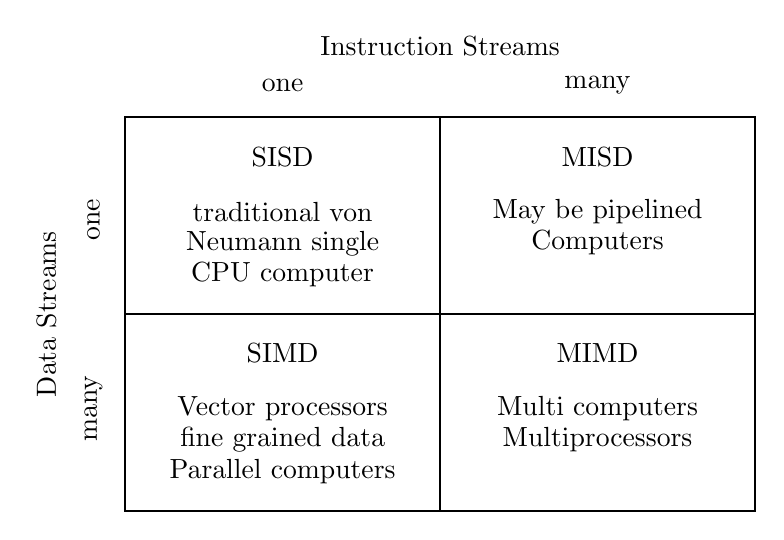
\begin{tikzpicture}
                    % Draw the grid lines
                    \draw[thick] (0,0) rectangle (8,5);
                    \draw[thick] (0,2.5) -- (8,2.5);
                    \draw[thick] (4,0) -- (4,5);
                    
                    % Add labels for SISD, SIMD, MISD, MIMD
                    \node at (2,4.5) {{\bold SISD}};
                    \node at (6,4.5) {{\bold MISD}};
                    \node at (2,2) {{\bold SIMD}};
                    \node at (6,2) {{\bold MIMD}};
                    
                    % Add descriptions for each category
                    \node at (2,3.8) {traditional von};
                    \node at (2,3.4) {Neumann single};
                    \node at (2,3) {CPU computer};
                    
                    \node at (6,3.8) {May be pipelined};
                    \node at (6,3.4) {Computers};
                    
                    \node at (2,1.3) {Vector processors};
                    \node at (2,0.9) {fine grained data};
                    \node at (2,0.5) {Parallel computers};
                    
                    \node at (6,1.3) {Multi computers};
                    \node at (6,0.9) {Multiprocessors};
                    
                    % Label axes
                    \node[rotate=90] at (-1,2.5) {Data Streams};
                    \node[rotate=90] at (-0.4,3.7) {one};
                    \node[rotate=90] at (-0.4,1.3) {many};
                    
                    \node at (2,5.4) {one};
                    \node at (6,5.4) {many};
                    \node at (4,5.9) {Instruction Streams};
                    
                \end{tikzpicture}
                
                \caption{A comparison between SISD, MISD, SIMD, and MIMD architectures}
            
            \end{figure}

            \subsection{SISD Architecture}

                \begin{wrapfigure}{r}{0.5\textwidth}

                    \centering

                    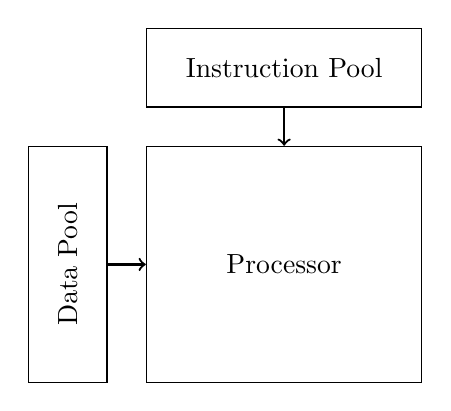
\begin{tikzpicture}

                            % Data Pool
                            \node[draw, minimum width=3cm, minimum height=1cm, rotate=90]  (data) at (0.25,0) {Data Pool};

                            % Instruction Pool
                            \node[draw, minimum width=3.5cm, minimum height=1cm] (instruction) at (3,2.5) {Instruction Pool};

                            % Processor
                            \node[draw, minimum width=3.5cm, minimum height=3cm] (processor) at (3,0) {{\bold Processor}};

                            % Arrows
                            \draw[thick, ->] (data.south) -- (processor.west);
                            \draw[thick, ->] (instruction.south) -- (processor.north);

                    \end{tikzpicture}

                    \caption{A conceptual diagram of SISD architecture.}

                \end{wrapfigure}

                The Single Instruction Single Data (SISD) architecture, introduced by John von Neumann in the late 1940s, processes one instruction at a time over a single data stream. This sequential nature means it doesn't support parallel processing, requiring only one processor to execute the tasks.

                An SISD computing system is a uniprocessor machine which is capable of executing a single instruction, operating on a single data stream. In SISD, machine instructions are processed in a sequential manner and computers adopting this model are popularly called sequential computers. Most conventional computers have SISD architecture. All the instructions and data to be processed have to be stored in primary memory.

                In the SISD model, the algorithm works in a serial fashion. For example, to sum a sequence of $n$ numbers, the algorithm accesses the memory $n$ times and performs $n−1$ additions. The time complexity for this approach can be expressed as:
        
                $$O(n)$$

                Where:

                \begin{itemize}
                    
                    \item $n$: The number of elements to process.

                    \item $O(n)$: Reflects that the algorithm's running time scales linearly with the size of the input.

                \end{itemize}

                In this architecture, there is no room for parallelism, and each operation occurs sequentially, requiring every data element to be processed one at a time. For a sum operation on $n$ numbers:

                \begin{itemize}

                    \item Memory accesses: $n$ memory fetches.
                    \item Additions: $n−1$ addition operations.

                \end{itemize}

                Thus, the total computational complexity is linear, i.e., $O(n)$, representing the number of accesses and operations required to complete the task. For this type of architecture, the performance is highly dependent on the efficiency of the processor and memory access speed, as there is no way to split the workload across multiple processors.
                
            \subsection{MISD Architecture}

                \begin{wrapfigure}{r}{0.5\textwidth}
                
                \centering
                
                    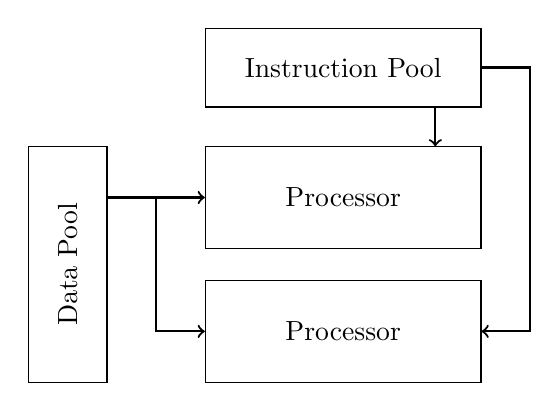
\begin{tikzpicture}

                            % Data Pool
                            \node[draw, minimum width=3cm, minimum height=1cm, rotate=90]  (data) at (-0.5,0) {Data Pool};

                            % Instruction Pool
                            \node[draw, minimum width=3.5cm, minimum height=1cm] (instruction) at (3,2.5) {Instruction Pool};

                            % Processors
                            \node[draw, minimum width=3.5cm, minimum height=1.3cm] (processor1) at (3,0.85) {{\bold Processor}};
                            \node[draw, minimum width=3.5cm, minimum height=1.3cm] (processor2) at (3,-0.85) {{\bold Processor}};

                            % Arrows
                            % Arrow from Data Pool to junction point
                            \draw[thick, ->] (0,0.85) -- (processor1.west);

                            % Arrow from junction point to Processor2
                            \draw[thick, ->] (0.625, 0.85) -- (0.625, -0.85) -- (processor2.west);

                            % Arrow from Instruction Pool to Processor1 (straight)
                            \draw[thick, ->] (4.17,2) -- (4.17,1.5);

                            % Arrow from Instruction Pool to Processor2 (broken path)
                            \draw[thick, ->] (instruction.east) -- (5.375, 2.5) -- (5.375, -0.85) -- (processor2.east);

                    \end{tikzpicture}

                    \caption{A conceptual diagram of MISD architecture.}

                \end{wrapfigure}

                The Multiple Instruction Single Data (MISD) is a less common architecture where multiple processors execute different instructions but operate on the same data stream simultaneously. This approach is primarily used in specialized applications like fault-tolerant systems or systems requiring redundancy. The MISD model is structured to handle cases where having multiple processors work on the same data but with different operations is crucial.

                In MISD architecture, each processor has its own control unit that dictates the operations performed. Unlike SIMD, which focuses on parallel data processing, MISD involves parallel instruction execution on a single data stream. To illustrate, imagine a real-time safety system where different sensors provide data that multiple processors analyze for distinct purposes:

                \begin{itemize}
                    
                    \item {\bold Processor 1} checks if the temperature is within a safe range.
                
                    \item {\bold Processor 2} monitors the pressure of the system.

                    \item {\bold Processor 3} assesses voltage levels.

                \end{itemize}

                All processors work on the same data stream from the sensors but perform different tasks to ensure system reliability and fault tolerance. If any processor detects a problem, the system can react accordingly to prevent failure.

                In a typical MISD system:

                \begin{itemize}

                    \item Multiple processors (N) receive the same input data simultaneously.

                    \item Each processor is responsible for executing a unique instruction on that shared data stream.

                    \item The processors operate in parallel, but the parallelism applies to the instruction execution, not to the data.

                \end{itemize}

                This kind of architecture is rare due to its niche applicability, often used in scenarios where redundancy is crucial, such as avionics or control systems, where the same data needs to be processed in multiple ways to ensure accuracy and safety.

                The time complexity of an MISD system depends heavily on the operations performed by each processor. Each processor runs independently, and the overall time to process the data is determined by the slowest processor, similar to SISD's sequential operation but distributed across different instruction sets.

                For N processors with execution times $T_1, T_2, \dots, T_N$, the overall time complexity is governed by the maximum time:

                $$T_{total}=max(T_1, T_2, \dots, T_N)$$

                This means the overall system performance is constrained by the processor taking the longest to complete its task.

                The Single Instruction Multiple Data (SIMD) architecture enables a single instruction to operate simultaneously across multiple data streams. In this model, one instruction, such as an addition or comparison, is applied to different sets of data in parallel, which significantly enhances processing efficiency.

                In an SIMD system, there are N identical processors, all controlled by a single stream of instructions from a central control unit. Each processor executes the same instruction but operates on its own separate data stream. Therefore, N data streams exist, with one data stream assigned to each processor.

                Communication between processors for data transfer in SIMD computers can occur in two main ways:

                \begin{enumerate}
                    
                    \item {\bold Shared memory:} All processors access a common memory space to fetch or store data. In Shared-Memory (SM) SIMD computers, the communication between processors occurs through a shared memory space. This model is often referred to as the Parallel Random-Access Machine (PRAM) model, where multiple processors work in parallel, and data exchange happens via common memory access.

                    When a processor (say {\bold processor i}) wants to send data to another processor ({\bold processor j}), the process follows two key steps:

                    \begin{enumerate}
                        
                        \item {\bold Processor i} writes the data into a known location in the shared memory, which {\bold processor j} can access.

                        \item {\bold Processor j} then reads the data from that specific location.
                        
                    \end{enumerate}

                    SIMD shared-memory computers are categorized based on how processors can concurrently access the same memory location. These categories determine how simultaneous read and write operations are handled, as follows:

                    \begin{itemize}
                        
                        \item {\bold Exclusive-Read, Exclusive-Write (EREW):} No two processors can read from or write to the same memory location at the same time.

                        \item {\bold Concurrent-Read, Exclusive-Write (CREW):} Multiple processors can read from the same memory location simultaneously, but only one can write to a memory location at any given time.

                        \item {\bold Exclusive-Read, Concurrent-Write (ERCW):} Only one processor can read from a memory location at a time, but multiple processors can write to the same location simultaneously.

                        \item {\bold Concurrent-Read, Concurrent-Write (CRCW):} Both read and write operations can be performed by multiple processors on the same memory location simultaneously.

                    \end{itemize}

                    These categories define the degree of parallelism and the restrictions on data sharing among processors in a shared-memory SIMD system.

                    \item {\bold Interconnection networks:} A specialized network connects the processors to facilitate data transfer between them.

                \end{enumerate}

                SIMD architecture is particularly well-suited for tasks requiring parallel data processing, such as graphical computations or heavy workloads where operations need to be performed on multiple data elements simultaneously. For example, in image or video processing, SIMD can process multiple pixels or image sections in parallel, leading to a significant speedup in computation.
                
                \begin{tcolorbox}[colback=white, colframe=black!25, title=Example]
                    
                    Searching for element x in an unordered file with n distinct entries using different SIMD models.

                    \begin{minipage}{0.49\linewidth} % First
                        \footnotesize
                        \vspace{0.3cm}
                        \begin{tcolorbox}[colframe=white, size=small]

                            {\bold Using the EREW Model with N processors where $N\geq n$}
                            

                            Phase 1:
                            
                            Broadcasting the value of x to all processors in  $O(N\log N)$ time

                            \begin{itemize}
                                
                                \item Processor P1 sends x to P3 and P2 sends x to P4, and so on.
                                \item This process continues until all processors have the value x.

                            \end{itemize}

                            Phase 2:
                            
                            Simultaneous search in sub-files by processors in $O(\frac{N}{n})$ time.
                            
                            \begin{itemize}
                                
                                \item Processor P1 searches the first $\frac{n}{N}$ data.
                                \item Processor P2 searches the second $\frac{n}{N}$ data.
                                \item And so on for all N processors.

                            \end{itemize}

                            Initially, F is set to false. The first processor to find x sets F to true. All processors check F at each step, and if F becomes true, the search ends. The broadcast of F takes $O(\log N)$ time per step.
                            In the worst case, the EREW model requires $+ O(N\log N(N \log(\frac{N}{n})))$ time.
                        \end{tcolorbox}
                    \end{minipage}
                    \hfill
                    \begin{minipage}{0.49\linewidth} % Second
                        \footnotesize
                        \vspace{0.3cm}
                        \begin{tcolorbox}[colframe=white, size=small]

                            {\bold Using the CREW Model with N processors where $N\geq n$}


                            Phase 1:
                            
                            Broadcasting the value of x to all processors in parallel using a single write per memory location.

                            \begin{itemize}
                                
                                \item Since concurrent reads are allowed, all processors can read the value of x from a shared memory location at the same time, significantly speeding up the process.

                                \item This reduces the broadcast time to $O(\log N)$ since only one write operation is needed.

                            \end{itemize}

                            Phase 2:
                            
                            Simultaneous search in sub-files by processors in $O(\frac{N}{n})$ time.

                            \begin{itemize}
                                
                                \item Similar to the EREW model, P1 searches the first $\frac{n}{N}$ data, P2 searches the second, and so on.

                                \item As soon as one processor finds x, it updates F to true, and the search ends.

                            \end{itemize}

                            With concurrent reads, the worst-case time complexity is reduced to $N\log (\frac{N}{n})+O(\log N)$.

                        \end{tcolorbox}
                    \end{minipage}

                    \begin{minipage}{0.49\linewidth} % Thired
                        \footnotesize
                        \vspace{0.3cm}
                        \begin{tcolorbox}[colframe=white, size=small]

                            {\bold Using the ERCW Model with N processors where $N\geq n$}

                            Phase 1:
                            
                            Broadcasting x to all processors in $O(\log N)$ time.

                            \begin{itemize}
                                
                                \item Similar to CREW, all processors can read x from a shared location.

                            \end{itemize}

                            Phase 2:
                            
                            Simultaneous search in sub-files by processors in $O(\frac{N}{n})$ time.

                            \begin{itemize}
                                
                                \item Again, processors search different parts of the data in parallel.
                                
                                \item However, here multiple processors can concurrently write to the same memory location. If one processor finds x, it writes to the shared F location. Other processors can also attempt to write, but only one write will succeed.

                            \end{itemize}

                            With concurrent writes, the time complexity remains $+O(\log N(N \log(\frac{N}{n})))$, though write conflicts may slightly impact performance.

                        \end{tcolorbox}
                    \end{minipage}
                    \hfill
                    \begin{minipage}{0.49\linewidth} % Fourth
                        \footnotesize
                        \vspace{0.3cm}
                        \begin{tcolorbox}[colframe=white, size=small]
                            
                            {\bold Using the CRCW Model with N processors where $N\geq n$}

                            Phase 1:
                            
                            Broadcasting x to all processors in constant time $O(1)$.

                            \begin{itemize}
                                
                                \item In this model, both reads and writes are performed concurrently, so all processors can obtain the value of x simultaneously from the shared memory.

                            \end{itemize}

                            Phase 2:
                            
                            Simultaneous search in sub-files by processors in parallel.

                            \begin{itemize}
                                
                                \item Each processor searches its assigned portion of the data. Once a processor finds x, it writes true to F, and the search concludes. Since multiple writes are allowed at the same memory location, any processor finding x can update F without delay.

                            \end{itemize}
                            
                            The worst-case time complexity for CRCW is minimized to $O(\frac{N}{n})$ because concurrent reading and writing reduce the overhead. 
                        
                        \end{tcolorbox}
                    \end{minipage}
                
                \end{tcolorbox}

                

\end{document}